\documentclass[border=2mm]{standalone}
\usepackage[usenames,dvipsnames]{xcolor}
\usepackage{tikz}

\newcommand{\cc}{c\nolinebreak\hspace{-.05em}\raisebox{.2ex}{\tiny\bf +}\nolinebreak\hspace{-.10em}\raisebox{.2ex}{\tiny\bf +}}

\newcommand{\vardonut}[1]{
    \newcounter{num}
    \foreach \content/\size/\colour in {#1}
        \stepcounter{num};
    \foreach \content/\size/\colour [count=\i] in {#1}{
        \draw[white,very thick,top color=\colour!50!black, bottom color=\colour, shading angle={-90+360/\thenum/2+(\i-1)*360/\thenum}] 
        ({2*cos((\i-1)*360/\thenum)},{2*sin((\i-1)*360/\thenum)}) arc[radius = 2, start angle={(\i-1)*360/\thenum}, delta angle=360/\thenum] --
        ({(2+\size)*cos(\i*360/\thenum)},{(2+\size)*sin(\i*360/\thenum)}) arc[radius = {2+\size}, start angle={\i*360/\thenum}, delta angle=-360/\thenum] -- 
        cycle;
        \node[white,font=\large] at ({(\i-1)*360/\thenum+360/\thenum/2}:{\size/2+2}) {\content};
    }
}

\begin{document}
    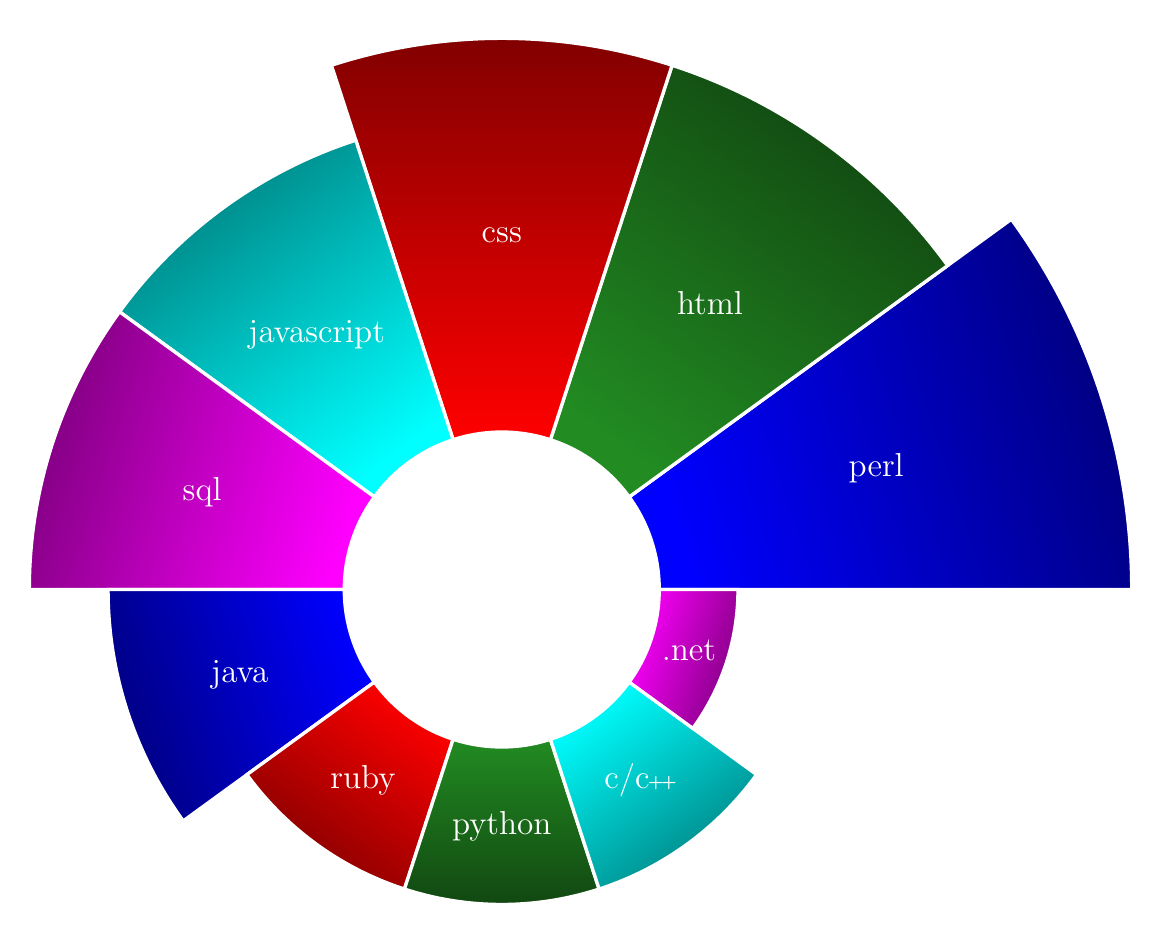
\begin{tikzpicture}
        \vardonut{perl/6/Blue, html/5/ForestGreen, css/5/Red, javascript/4/Cyan, sql/4/Magenta, java/3/Blue, ruby/2/Red, python/2/ForestGreen, {c/\cc}/2/Cyan, .net/1/Magenta}
    \end{tikzpicture}
\end{document}
